\section{Broadcast Jamming Resistant Communication}
\subsection{Introduction}

\paragraph{Broadcast Communication}
\begin{itemize}
    \item One sender, many receivers. 
    \item Open system: new receivers may join/witdraw, Any receiver can listen (in contrast to multicast)
    \item E.g.: radio broadcast, navigation signals.
\end{itemize}

\paragraph{Attacks on Broadcast Communication}
\begin{itemize}
    \item For pairwise (unicast) communication only consider \textcolor{orange}{external attackers}
    \item For Broadcast communication consider \textcolor{orange}{external attackers} and \textcolor{orange}{internal attackers}
\end{itemize}

\paragraph{External Attackers on SS Techniques}
\begin{itemize}
    \item Does not know spreading code / hopping sequence
    \item Partial-band attacker can still jam. Example: FHSS
\end{itemize}

\paragraph{Internal Attacker on SS Techniques}
\begin{itemize}
    \item Legitimate receiver knows the spreading code and its synchronization!Can misuse this for jamming
    \item Group keys do not prevent this attack!
\end{itemize}

\paragraph{Anti-Jamming Broadcast}
\begin{itemize}
    \item Problem: Base station (BS) needs to broadcast an (authenticated/confidential) message to a large nr. of receivers in an anti-jamming manner.
    \item Desirable Properties: 
    \begin{itemize}
        \item Detect/ prevent jamming
        \item Support a flexible nr of receivers
        \item Tolerate a certain fraction of malicious receivers
    \end{itemize}
\end{itemize}

\subsection{Solutions based on Shared Keys}
The following solutions rely on a shared secret, and thus follow the multicast strategy rather than broadcast.

\subsubsection{Broadcast anti-jamming based on frequency hopping (FHSS)}
Coding method provides protection against malicious receivers [Desmedt et al.]
\begin{itemize}
    \item Base station transmits the same signal simultaneously on multiple frequencies
    \item Each receiver listens to a subset of these frequencies at a given time
    \item Threshold scheme: provides protection against up to j-1 colluding receivers
    \item Public Channel allocation Table: Defines the subset of channels where each receiver $R_i$ is listening. j-i receivers do not cover all channels of any other receiver. Set coverage problem.
    \item Secret Frequency Allocation Table: The actual frequencies are secret. Created and updated via a pseudo-noise generator.
    \item The assigned frequencies can be distributed over a broad, non-continuous frequency band.
    \item Multicast solution 
    \item \textcolor{green}{Successful if:} The group of colluders consists of j-1 or fewer members.
\end{itemize}

\begin{minipage}{\linewidth}
    \centering      
    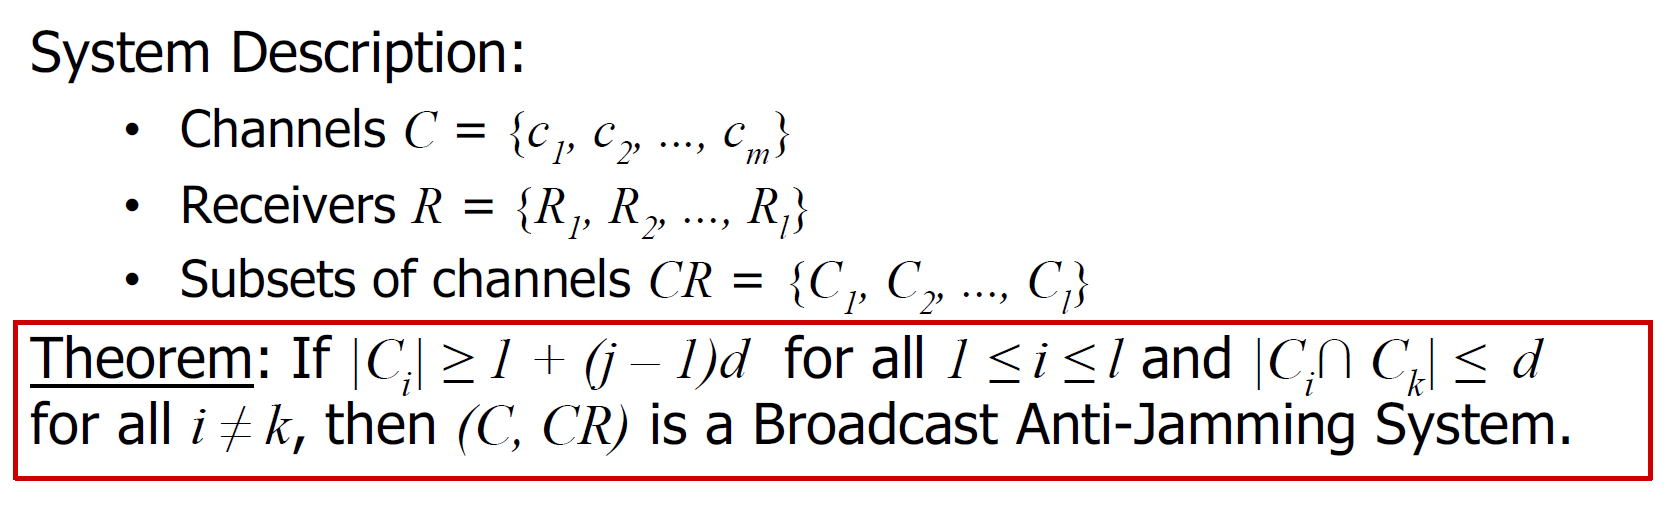
\includegraphics[width=\linewidth]{Figures/L3_Theorem.PNG} 
\end{minipage}

\subsubsection{Dynamic Jamming Mitigation}
Broadcast anti-jamming based on DSSS [Chiang and Hu]
\begin{itemize}
    \item Counteract jamming by using a balanced binary key tree. Each node corresponds to a spreading code. Each user $N_i$ is assigned to a leaf and knows all codes on the path from the root.
    \item The BS transmits on... 
    \begin{itemize}
        \item a disjoint cover of codes, i.e. all users can decode using exactly one code (of their many codes they got). Not necessarily the leaf node b.c. nodes on the path reach multiple users, so base station does not have to send with seperate code for all users.
        \item a set of test codes 
    \end{itemize}
    \item If a user receives a message on a test code but not on the corresponding detectable code, it reports jamming.
    \item Splitting and reforming the tree allows the transmitter to send each transmission on $\leq 2j + 1$ codes, where j is the (expected upper) nr of jammers.
    \item Requires highly flexible base station (sending and receiving on a potentially large nr of codes) and feedback channels. Not applicable to unidirectional broadcast.
    \item Nr of secrets grows with nr of receivers.
    \item multicast solution 
\end{itemize}

\subsection{Broadcast Anti-Jamming Techniques Without Shared Secrets}

\textbf{Goal:} BS broadcasts authenticated message to a large nr of unknown/untrusted receivers in an anti-jamming manner.\\
\textbf{Applications:} alarm broadcast, navigation signals, ...\\
\textbf{Problems:} 
    \begin{itemize}
        \item The prior schemes (Desmedt, Chiang) do not work for unknown receivers (they need a shared secret) and also Public-key crypto does not help.
        \item Anti-Jamming Key Establishment depends on jamming-resistant communication.
    \end{itemize}
\textbf{Solution} Sender uses random hopping sequences / spreading codes unknown to the receiver. The attacker cannot predict which channels will be used (neither can the receiver). Latency and Throughput will probably decrease through this procedure (UDSSS definitely has reduced latency compared to DSSS).\\
\textbf{Attacker Model:} 
\begin{itemize}
    \item goal: prevent communication
    \item actions: Jam, Insert, Modify
\end{itemize}

\subsubsection{Uncoordinated Frequency Hopping (UFH)}

\begin{minipage}{\linewidth}
    \centering      
    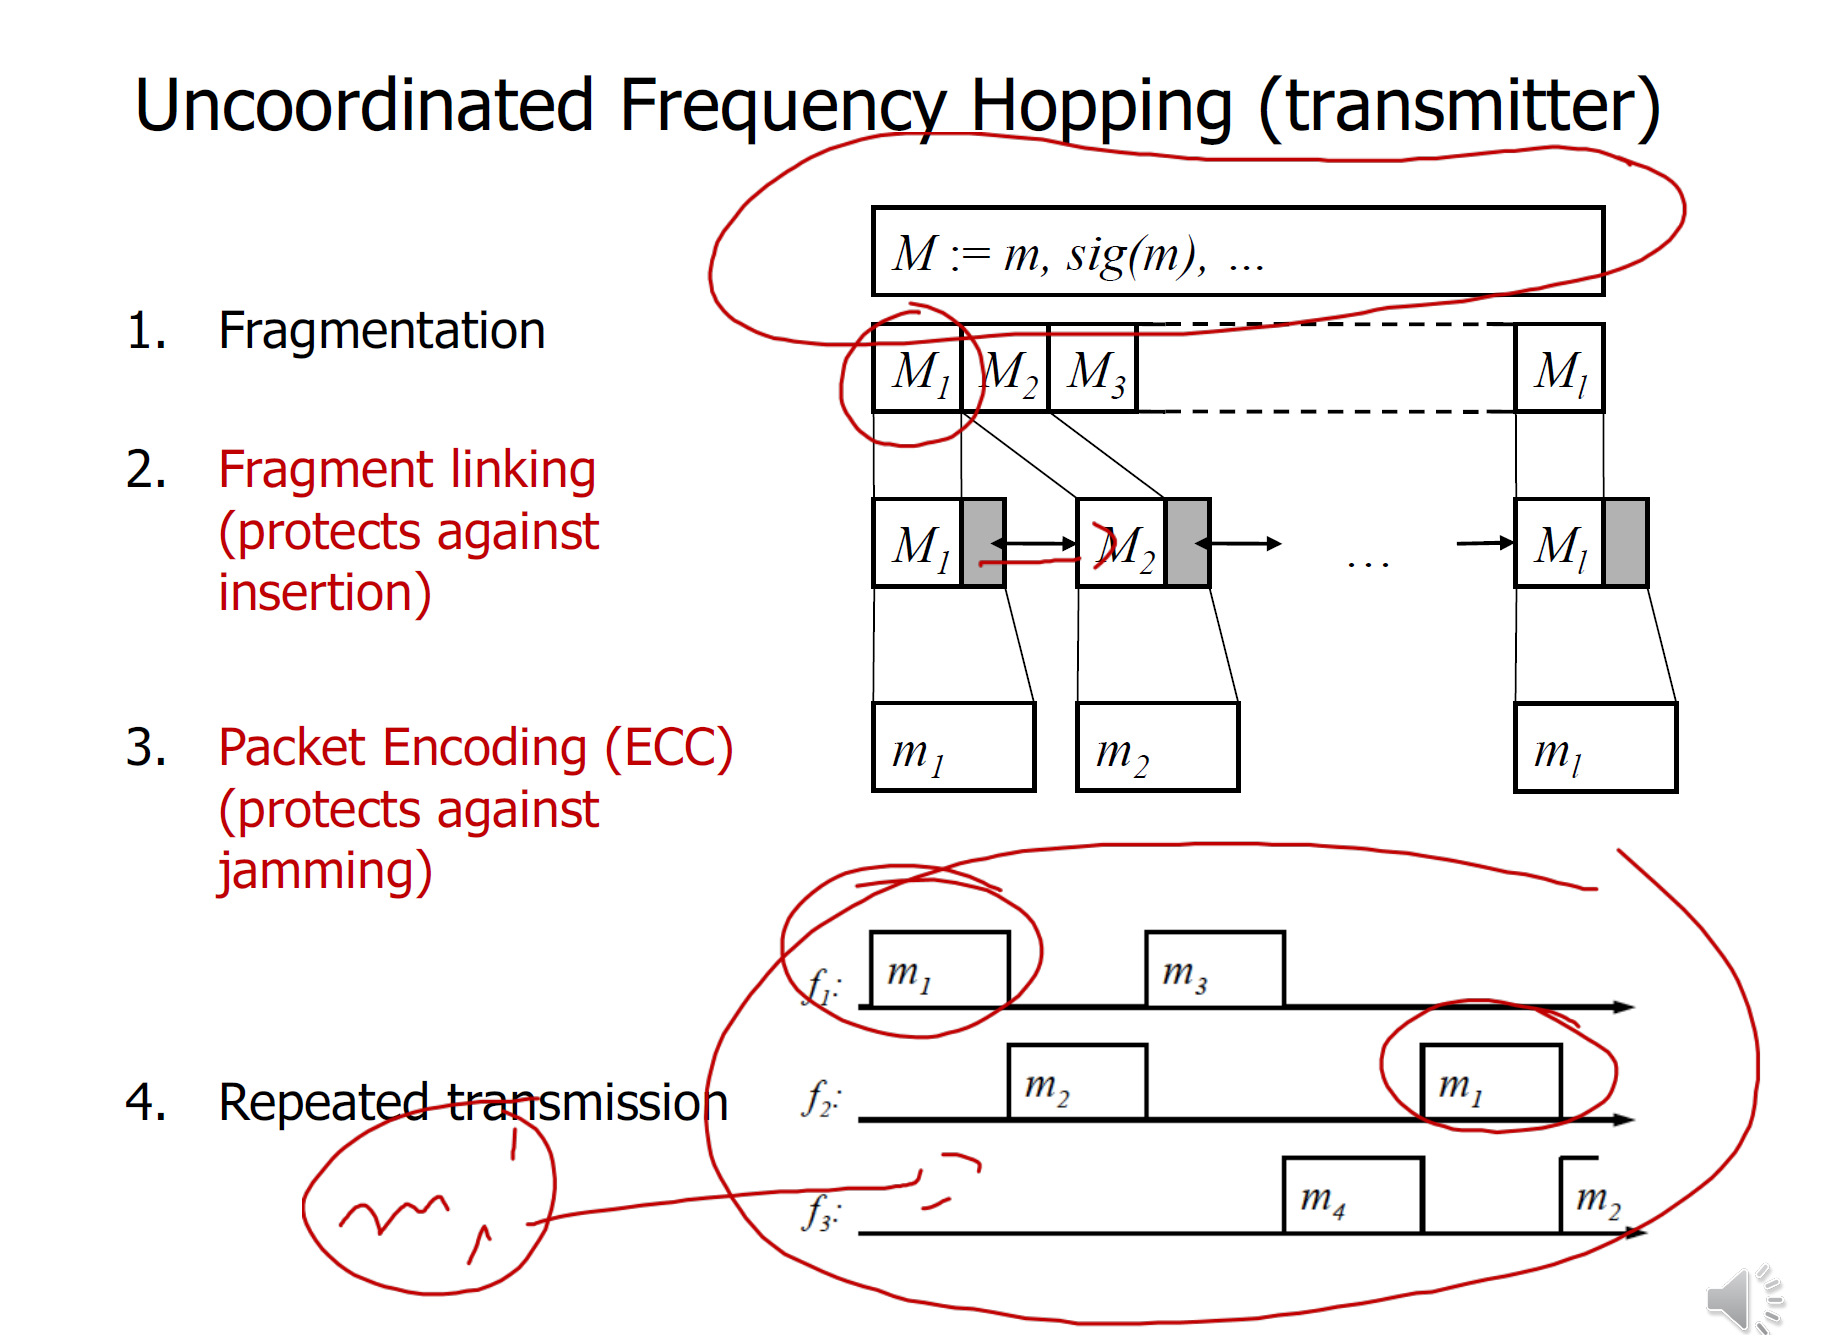
\includegraphics[width=\linewidth]{Figures/L3_ufh_sender.PNG} 
\end{minipage}
\begin{minipage}{\linewidth}
    \centering      
    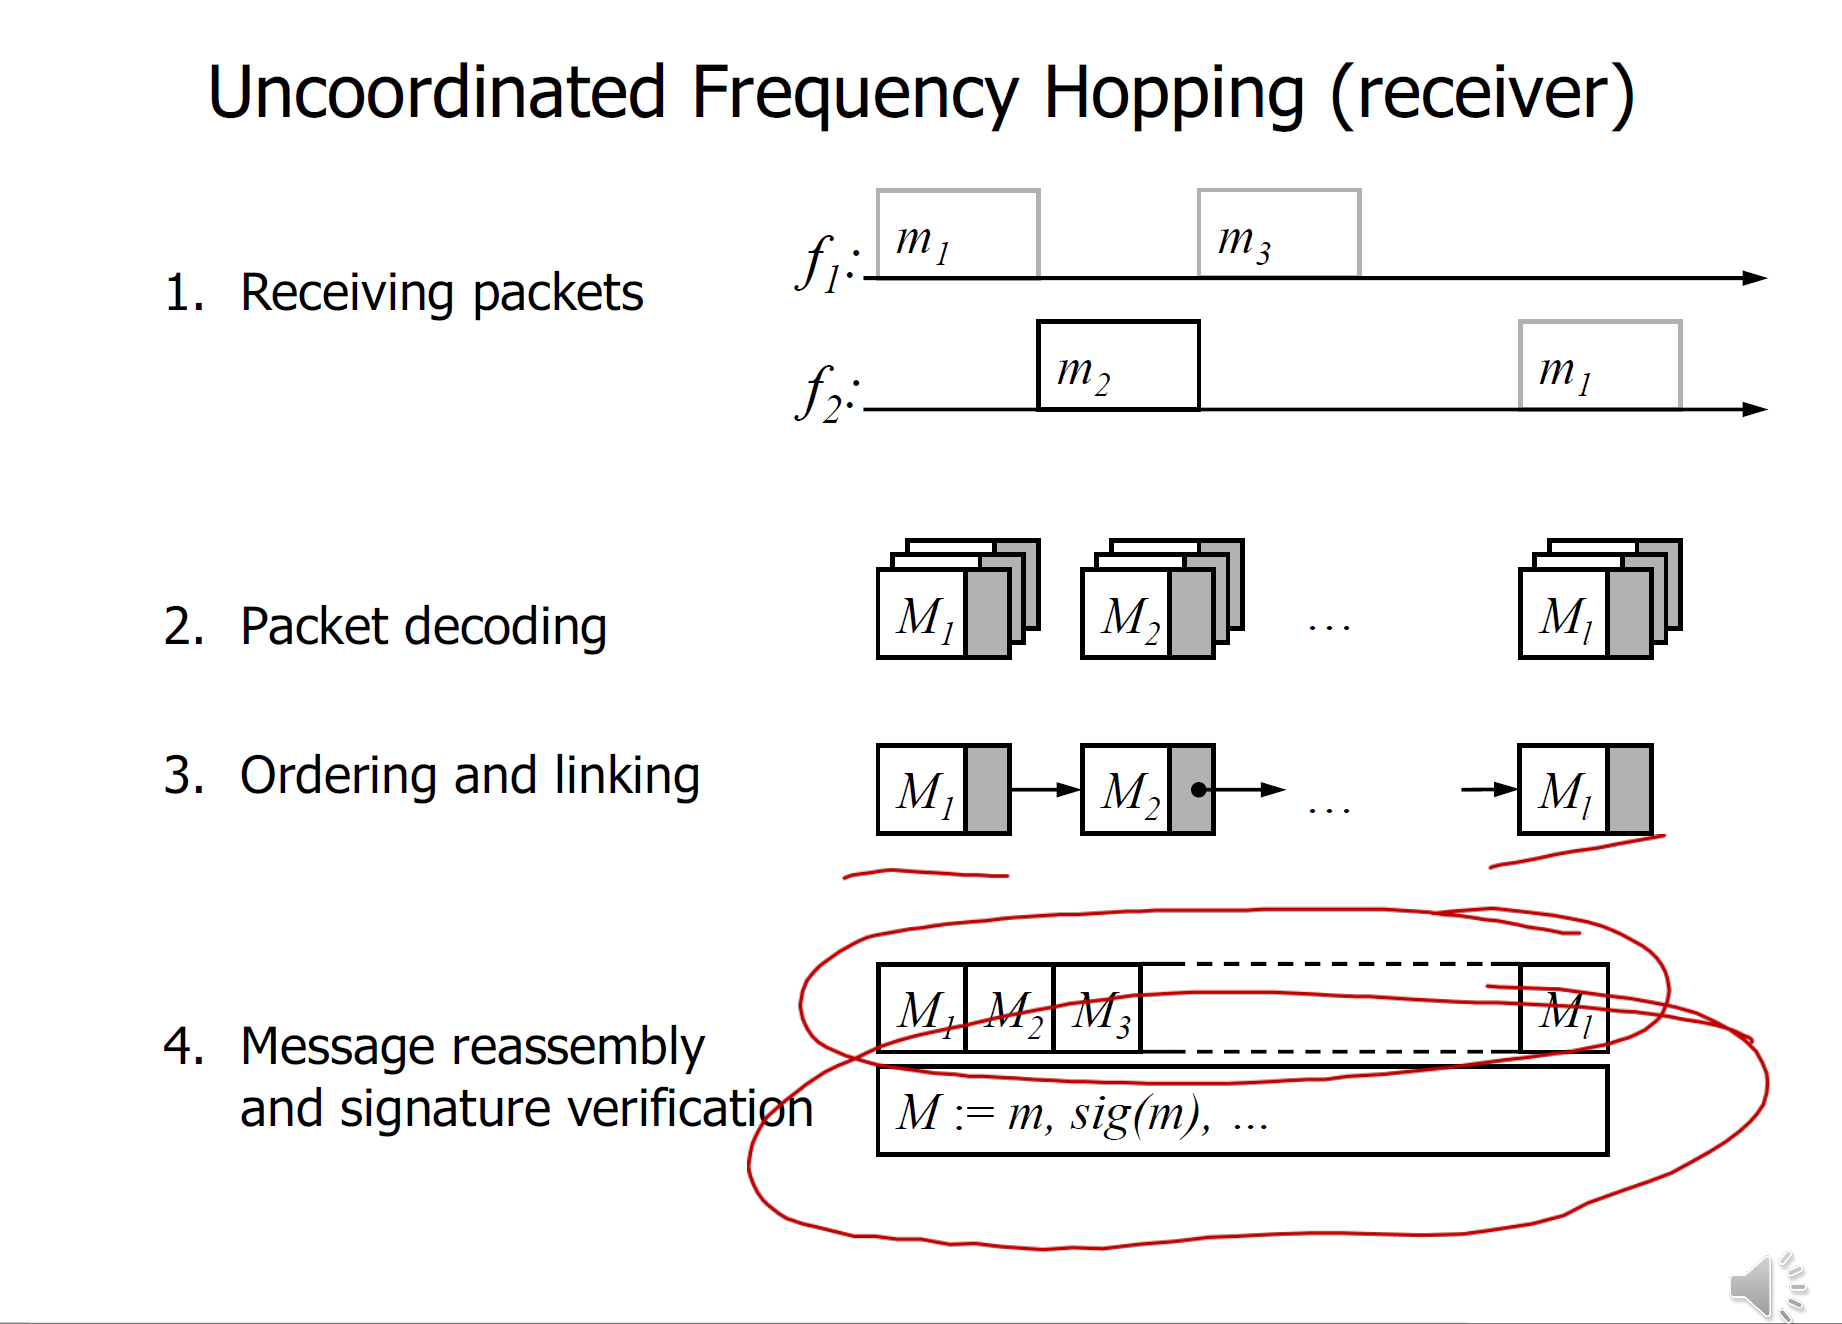
\includegraphics[width=\linewidth]{Figures/L3_ufh_receiver.PNG} 
\end{minipage}
\textbf{Throughput:} Can be improved by using broadband receivers.\\
\textbf{\textcolor{red}{Problem:}} Fragments are not individually authenticated, thus we need cryptographic fragment linking (Hash linking, One-way Acccumulators, Short signatures) and signature verification to achieve message integrity. If not Attacker can perform a DoS attack by increasing the space over which receiver has to try to link fragments, by inserting fake fragments. Signatures and accumulators are better than hash linking b.c. they reduce this search space!

\subsubsection{Uncoordinated Direct Sequence Spread Spectrum (UDSSS)}
\textbf{Basic Idea:} Public code set C composed of n code sequences, each of which is composed of l spreading codes containing N chips. Successful despreading requires to hit the correct spreading sequence and the correct synchronization.
\begin{minipage}{\linewidth}
    \centering      
    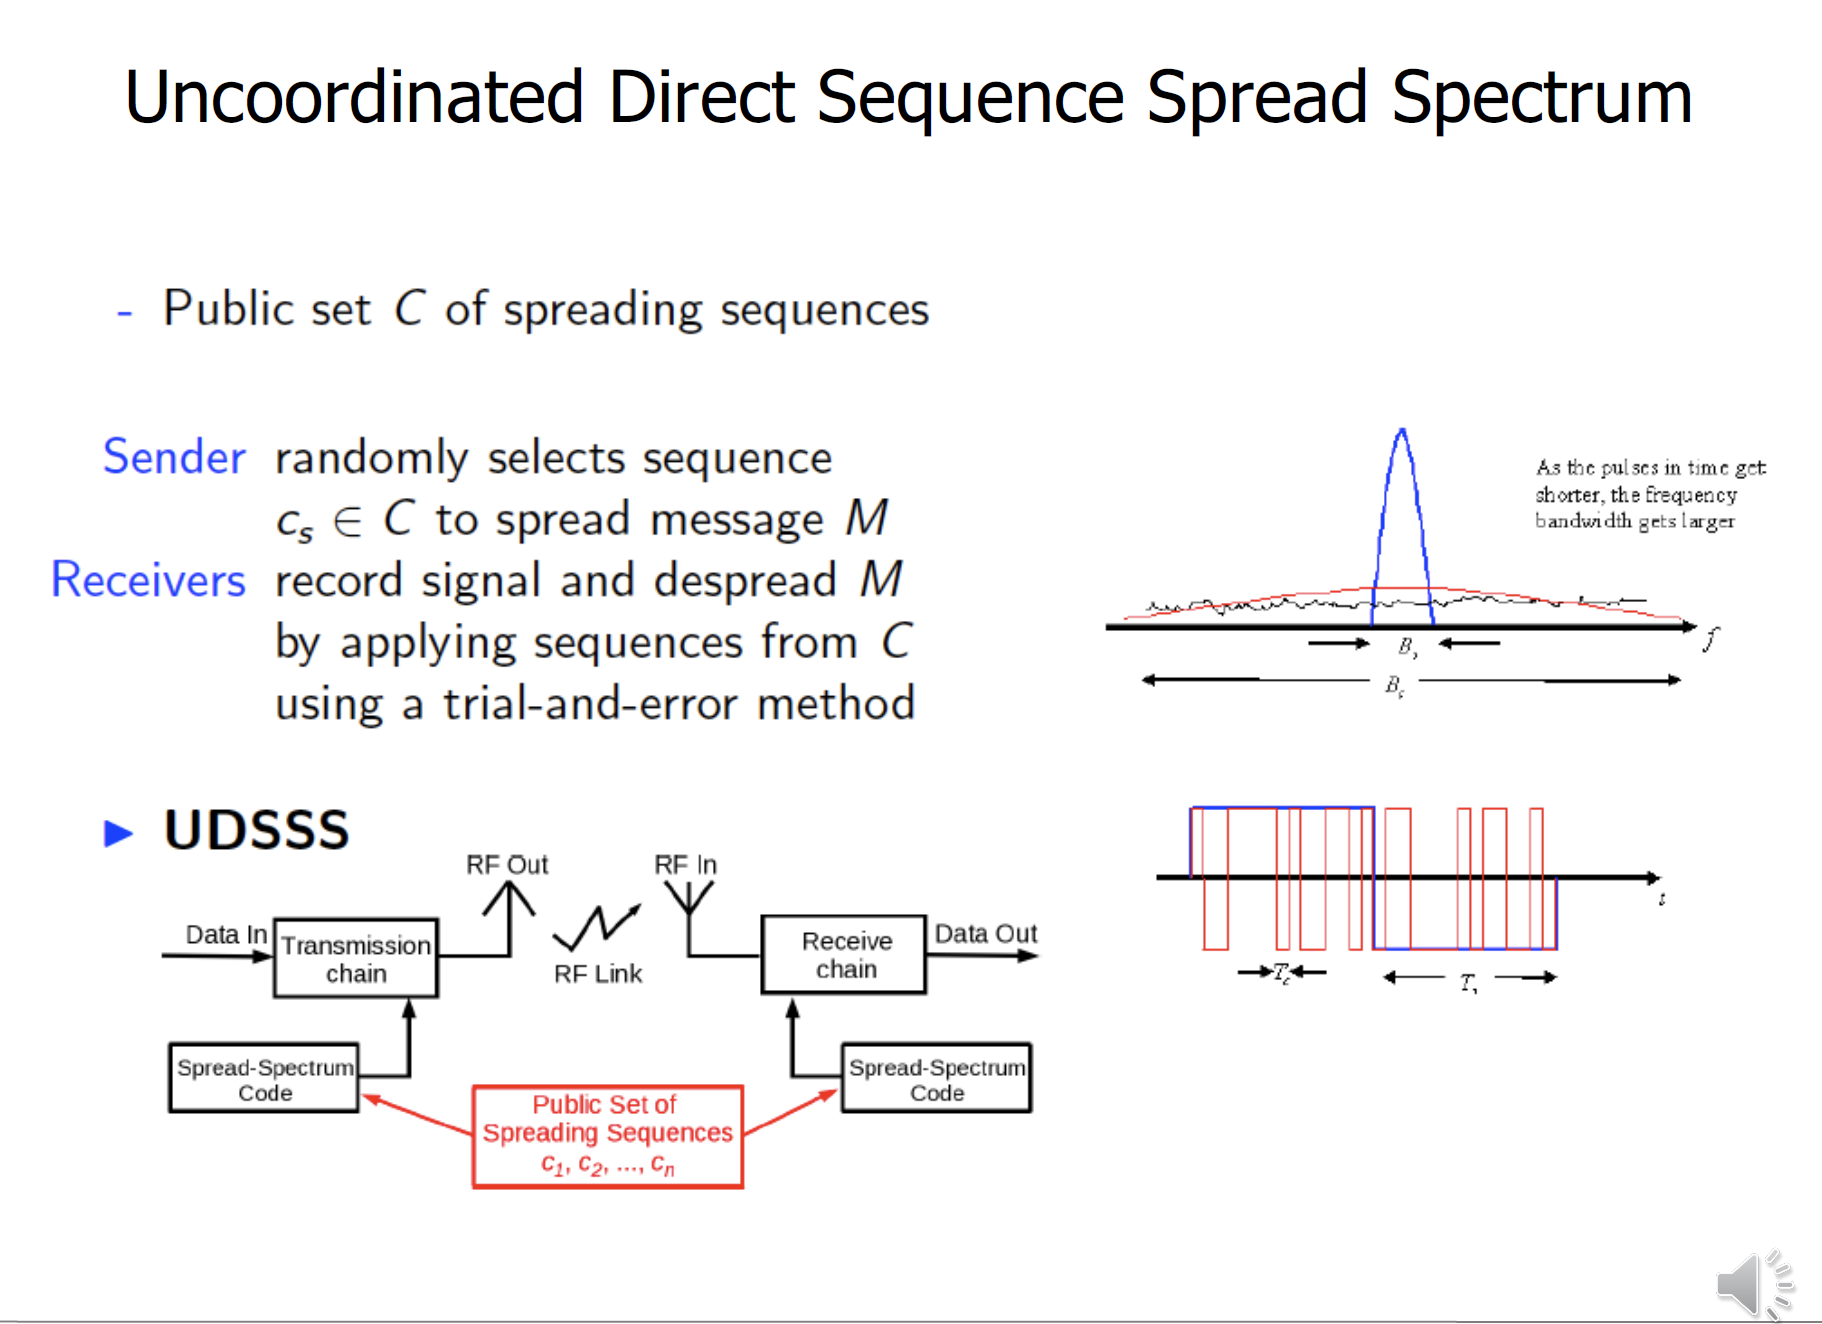
\includegraphics[width=\linewidth]{Figures/L3_udsss.PNG} 
\end{minipage}
\textbf{Message Repetitions:} due to both the lacking synchronizatino between sender and receivers and the possibility of successful jamming attacks.\\
\textbf{Throughput:} Can be improved by using parallelization.\\
\textbf{Further Optimization:} Use UDSSS to transmit the spreading key only. First transmit message M using a random spreading code K, then transmit the spreading code K using UDSSS. Smaller spreading code set, Quicker decoding, Longer messages and more flexible security level.\\
\textbf{Applications:} For positioning and/or time-synchroization

\subsection{Application of Anti-Jamming Techniques to Key Establishement}

\paragraph{Problems with Key Establishement:}
\begin{itemize}
    \item Pre-sharing symmetric keys: Efficient but a trusted third party is needed, suffers from network dynamics problems (new nodes joining, key revocation, key compromise)
    \item Key establishment: Based on public-key crypto (RSA, DH), requires reliable communication.
\end{itemize}

\paragraph{Key Idea:} break the anti-jamming/key-establishment dependency cycle by using UFH.

